%  http://latex-beamer.sourceforge.net/

%\documentclass[landscape]{foils}

%\documentclass{beamer}
%\documentclass[handout]{beamer}     % TO PRINT PRESENTATION HANDOUT
\documentclass[xcolor=dvipsnames]{beamer}  % ALLOWS CHANGE IN COLOR

\usepackage{pifont} %para tener la ballot cross \ding{55}

\usepackage{beamerthemesplit}
\usepackage{url}
\usepackage{ae} % or {zefonts}
\usepackage[T1]{fontenc}
\usepackage[ansinew]{inputenc}
\usepackage[spanish,es-nodecimaldot]{babel}

\usepackage{amsmath}

\usepackage{graphicx}
\graphicspath{"../graphs/"}
\usepackage{color}
%\usepackage[colorlinks]{hyperref} % beamer loads this by default, needed only to change default behavior? 
\usepackage{tikz} % Easier syntax to draw pgf files (invokes pgf automatically)
\usetikzlibrary{arrows,shapes.geometric}

\usepackage{tabulary} % automatic column length in tables with long text string
%% use LRJC for auto, and lrjc for normal column width
\setlength\tymin{10pt}       %% change behavior, see p. 254 LaTeX companion
\setlength\tymax{\maxdimen}  %% change behavior, see p. 254 LaTeX companion

\usepackage{multirow} %allows multiple rows in tables

%\usecolortheme{crane}     %Color yellow
%\usetheme{Warsaw}
\usecolortheme[named=Gray]{structure}

\useoutertheme[footline=empty]{}  % PUTS COLORED LINE AT FOOT WITH TITLE, AUTHOR, PAGE, etc
%\usetheme{Berkeley}
\usetheme[height=7mm]{Rochester}
\setbeamertemplate{items}[ball]   % ITEMS IN 3D BALLS (alt CIRCLES)
\setbeamertemplate{navigation symbols}{}  % DROPS NAVIGATION ICONS
\setbeamertemplate{blocks}[rounded][shadow=true]

%\setbeamertemplate{footline} {
%    \begin{beamercolorbox}{section in head/foot}
%    \insertsectionnavigationhorizontal{\paperwidth}{}{plus1filll
%    \insertframenumber}
%    \end{beamercolorbox}
%}

%\setbeamertemplate{navigation symbols}{\insertslidenavigationsymbol,
%\insertdocnavigationsymbol} \setbeamertemplate{footline} {
%    \begin{beamercolorbox}{section in head/foot}
%    \insertsectionnavigationhorizontal{\paperwidth}{}{plus1filll
%    \insertframenumber}
%    \end{beamercolorbox}
%}

\setbeamercovered{transparent}
\setbeamertemplate{caption}{\insertcaption}
\setbeamertemplate{footline}[frame number] % adds slide number, overrides split footer with authors/title that the theme uses

\tikzstyle{nodo} = [circle, draw=black, fill=white, text=black]
\tikzstyle{end} = [circle, minimum width=3pt,fill, inner sep=0pt]

\usepackage{arydshln}         % dashed lines in tables (usage: \hdashline, \cdashline{3-4}, 
                              %see http://tex.stackexchange.com/questions/20140/can-a-table-include-a-horizontal-dashed-line)
                              % must be loaded AFTER dcolumn, 
                              %see http://tex.stackexchange.com/questions/12672/which-tabular-packages-do-which-tasks-and-which-packages-



\title[Malapportionment \& bias]{The effects of malapportionment, turnout, \\ and gerrymandering in Mexico's \\ mixed-member system}
%\subtitle{Party bias and responsiveness in Mexico}
\author[Magar, Altman, McDonald, Trelles]{E. Magar\inst{1} \and M. Altman\inst{2} \and M.P. McDonald\inst{3} \and A. Trelles\inst{4}}
\institute[ITAM-MIT-UFG-Pitt]{\inst{1} ITAM \and 
                              \inst{2} MIT \and
                              \inst{3} UF \and
                              \inst{4} Pitt}
%\address{}
\date[18apr15]{MPSA annual meeting \\ 4/18/15}

\begin{document}

%%%%%%%%%%%%%%%%%%%%%%%%%%%%%%%%%%%%%%%%%%%%%%%%%%%%%%%%%%%%%%%%%%%%%%%%%%%%%%%%%%%%%%%%%%%%

\frame[plain]{\titlepage}

%%%%%%%%%%%%%%%%%%%%%%%%%%%%%%%%%%%%%%%%%%%%%%%%%%%%%%%%%%%%%%%%%%%%%%%%%%%%%%%%%%%%%%%%%%%%
\frame {
    \frametitle{Background on Mexico}

\begin{itemize}

%\item 32 states, 2.5k municipalities, 67k electoral \emph{secciones}

\item Hegemonic party 1929--1997 

\item Three major parties: \begin{tabular}{ccc} PRD & PRI & PAN \\ left & & right \end{tabular} and minors

\item Lower chamber of Congress elected every 3 years, \\ concurrent w presidential race every 6 years

\item Mixed system: 300 SMD + 200 PR seats

\item Single-term limits removed in 2018

\item Autonomous regulator (IFE) organizes elections and redistricting

\end{itemize}
}
%%%%%%%%%%%%%%%%%%%%%%%%%%%%%%%%%%%%%%%%%%%%%%%%%%%%%%%%%%%%%%%%%%%%%%%%%%%%%%%%%%%%%%%%%%%%
\frame {                      % SLIDE
    \frametitle{Questions}

Did 1997 reform remove \textbf{party bias} in representation? 

\begin{itemize}
\item Potential problem wherever districts are drawn to allocate seats (Tufte 1973, Johnston 2002)
\end{itemize}

\bigskip

If party bias remains, what \textbf{factors} drive it?

\begin{itemize}
\item Do parties use redistricting in their advantage? 
\item How do demographic shifts over time affect parties? 
\item Turnout differentials?
\end{itemize}
%(Grofman et al.\ 1997)

\pause

\bigskip

\begin{block}{Answers}

\begin{enumerate}
\item Persistent bias against the right 
\item Components of bias often cancel each other 
\end{enumerate}

\end{block}
}
%%%%%%%%%%%%%%%%%%%%%%%%%%%%%%%%%%%%%%%%%%%%%%%%%%%%%%%%%%%%%%%%%%%%%%%%%%%%%%%%%%%%%%%%%%%%
\frame {                      % SLIDE
    \frametitle{What is party bias}

\begin{center}
It is the excess/defect seat share that a \\ party with half of the votes gets: \\ 
\medskip
($s$ | $v$=.5) -- .5
\end{center}

\pause

\bigskip

\begin{itemize}
\item Two-party system
\item Constant-sum game
\item Vote wasting: too-concentrated large party  or \\ too-dispersed small party  suffer bias \\ (Calvo\&Rodden 2015)
\end{itemize}



}
%%%%%%%%%%%%%%%%%%%%%%%%%%%%%%%%%%%%%%%%%%%%%%%%%%%%%%%%%%%%%%%%%%%%%%%%%%%%%%%%%%%%%%%%%%%%
\frame {                      % SLIDE
    \frametitle{Obstacle 1: measure party bias}

Fitting votes--seats curves: $s = f(v)$  \\ (Rae 1967, Tufte 1973, King\&Browning 1987)

 \begin{columns}[c]

 \column{.4\textwidth}
\centering

\medskip

\begin{equation*}
\frac{s}{1-s} = \lambda \left( \frac{v}{1-v} \right)^\rho
%$\text{logit}(s) = \ln(\lambda) + \rho \text{logit}(v)$
\end{equation*}

\column{.6\textwidth}

\begin{center}
   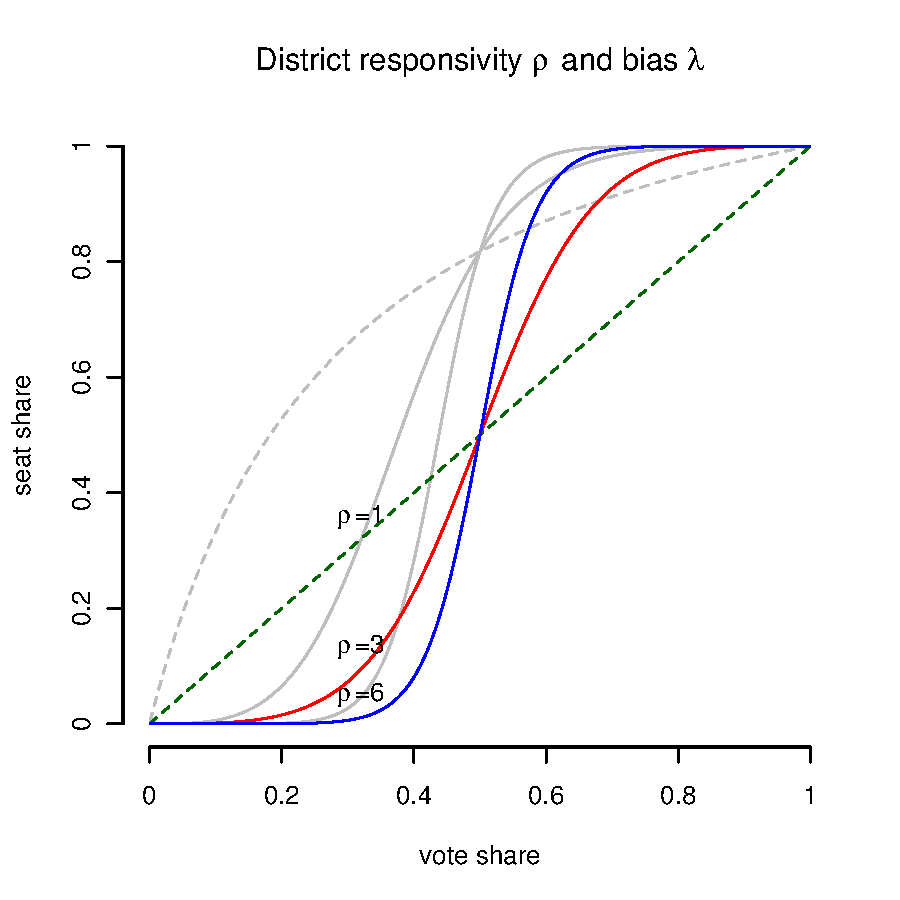
\includegraphics[width=6cm]{../../graphs/rhoLambdaExample.pdf} 
\end{center}

\end{columns}


}
%%%%%%%%%%%%%%%%%%%%%%%%%%%%%%%%%%%%%%%%%%%%%%%%%%%%%%%%%%%%%%%%%%%%%%%%%%%%%%%%%%%%%%%%%%%%
\frame {                      % SLIDE
    \frametitle{Three sources of party bias}


\newcommand{\mc}{\multicolumn}
\centering
% %\newcolumntype{d}[1]{D{.}{.}{#1}} % D column with 1 decimal spaces default, usage d{2} for two spaces
%\newcolumntype{d}{D{.}{.}{2}} % D column with space for 2 decimal spaces
%\begin{tabular}{lrdrrrrddrrrrdd}
\resizebox{\textwidth}{!}{
\begin{tabular}{lrrrrrrrrrrrrrr}
          &              &                  &  \mc{3}{c}{Raw votes}      &&  \mc{2}{c}{Vote shares}        && \mc{2}{c}{Seat shares}\\ \cline{4-6} \cline{8-9} \cline{11-12}
%         &  (d)         &    (c/d)         &  a        &  (b)  &  (c)   && \mc{1}{r}{a/c}&   b/c          \\
Districts &  Pop.        &\mc{1}{r}{Turnout}&  left     & right&  total  &&\mc{1}{r}{left}&\mc{1}{r}{right}&&\mc{1}{r}{left}&\mc{1}{r}{right}\\ \hline
\mc{9}{l}{~~\textbf{Gerrymandering}}                                                 && &     \\    
1 and 2   &  420         &   .5             &  147      &  63  &  210    &&   .\textbf{7} &   .\textbf{3}  && 1 & 0 \\
3, 4 and 5&  420         &   .5             &  84       &  126 &  210    &&   .\textbf{4} &   .\textbf{6}  && 0 & 1 \\ \hdashline
nationwide&  2100        &   .5             &  546      &  504 &  1050   &&   .52         &   .48          &&.4 &.6 \\ \hline
\mc{9}{l}{~~\textbf{Turnout}}                                                        && &     \\
1 and 2   &  420         &   .\textbf{70}   &  200      &  100 &  300    &&   .67         &   .33          && 1 & 0 \\
3, 4 and 5&  420         &   .\textbf{35}   &  50       &  100 &  150    &&   .33         &   .67          && 0 & 1 \\ \hdashline
nationwide&  2100        &   .5             &  550      &  500 &  1050   &&   .52         &   .48          &&.4 &.6 \\ \hline
\mc{9}{l}{~~\textbf{Malapportionment}}                                               && &     \\ 
1 and 2   & \textbf{600} &   .5             &  200      &  100 &  300    &&   .67         &   .33          && 1 & 0 \\
3, 4 and 5& \textbf{300} &   .5             &  50       &  100 &  150    &&   .33         &   .67          && 0 & 1 \\ \hdashline
nationwide&  2100        &   .5             &  550      &  500 &  1050   &&   .52         &   .48          &&.4 &.6 \\ \hline
\end{tabular}
}

}
%%%%%%%%%%%%%%%%%%%%%%%%%%%%%%%%%%%%%%%%%%%%%%%%%%%%%%%%%%%%%%%%%%%%%%%%%%%%%%%%%%%%%%%%%%%%
\frame {                      % SLIDE
    \frametitle{Obstacle 2: measure the sources of party bias}


\begin{block}{Grofman, Koetzle \& Brunell 1997:} 
Three additive components
\begin{tabular}{rl}
raw party bias~~=& gerrymandering (distributional) \\
      & + malapportionment \\
      & + turnout \\
\end{tabular}
\end{block}

\bigskip

\begin{enumerate}
\item Fitting votes--seats curve with $v$ yields \textbf{raw} party bias
\item with $\bar{v}$ yields the \textbf{gerrymandering}-based
\item with $\bar{w}$ yields gerrymandering + malapportionment
\end{enumerate}

\pause
    
\bigskip

$\rightarrow$ Subtract (3) -- (2) = \textbf{malapportionment}-based

$\rightarrow$ Subtract (1) -- (3) = \textbf{turnout}-based

}
%%%%%%%%%%%%%%%%%%%%%%%%%%%%%%%%%%%%%%%%%%%%%%%%%%%%%%%%%%%%%%%%%%%%%%%%%%%%%%%%%%%%%%%%%%%% 
\frame{                      % SLIDE
    \frametitle{Malapportionment is substantial}

\centering

%$RRI = \frac{1/\text{district size}}{300/\text{national population}} = \frac{Q}{\text{district size}}$
$RRI = \frac{Q}{\text{district size}}$

\bigskip

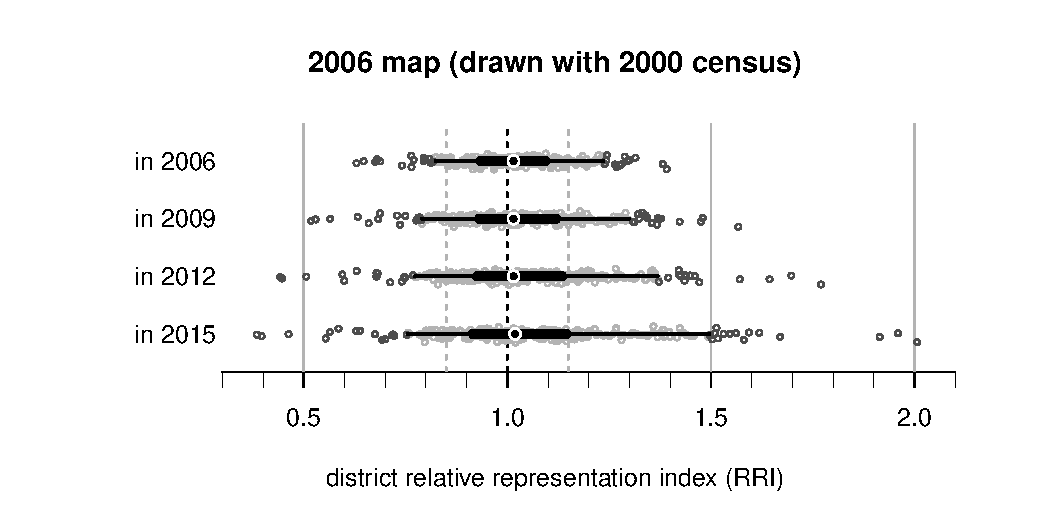
\includegraphics[width=.6\textwidth]{../../graphs/rrin0615d0.pdf} \\
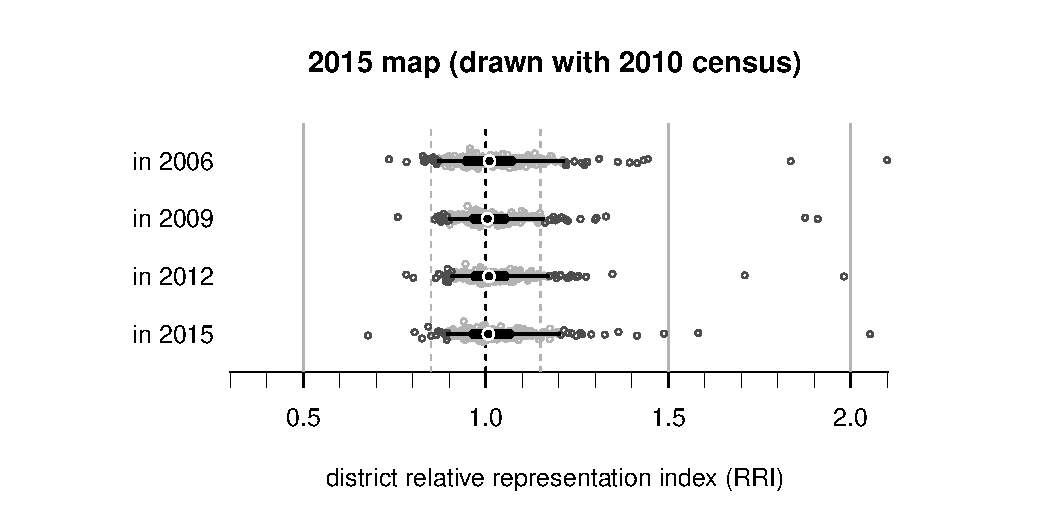
\includegraphics[width=.6\textwidth]{../../graphs/rrin0615d3.pdf} 


}
%%%%%%%%%%%%%%%%%%%%%%%%%%%%%%%%%%%%%%%%%%%%%%%%%%%%%%%%%%%%%%%%%%%%%%%%%%%%%%%%%%%%%%%%%%%%
\frame {                      % SLIDE
    \frametitle{Obstacle 3: a multiparty system}
King 1990: \begin{equation*}
 E(s_p) = \frac{e^{\lambda_p} v_p^\rho}{\sum_{q=1}^{P} e^{\lambda_q}  v_q^\rho}
\end{equation*}

\bigskip

Bias is expressed relative to a \\ baseline party (PRI in our case)
}
%%%%%%%%%%%%%%%%%%%%%%%%%%%%%%%%%%%%%%%%%%%%%%%%%%%%%%%%%%%%%%%%%%%%%%%%%%%%%%%%%%%%%%%%%%%%
\frame {                      % SLIDE
    \frametitle{Obstacle 4: small-N}
\begin{itemize}
\item Linzer 2012: approximates prob.\ distribution of national party vote returns from observed district outcomes (FMM)
\item Use to simulate many elections w Monte Carlo draws
\end{itemize}

\begin{center}
\begin{tabular}{cc}
   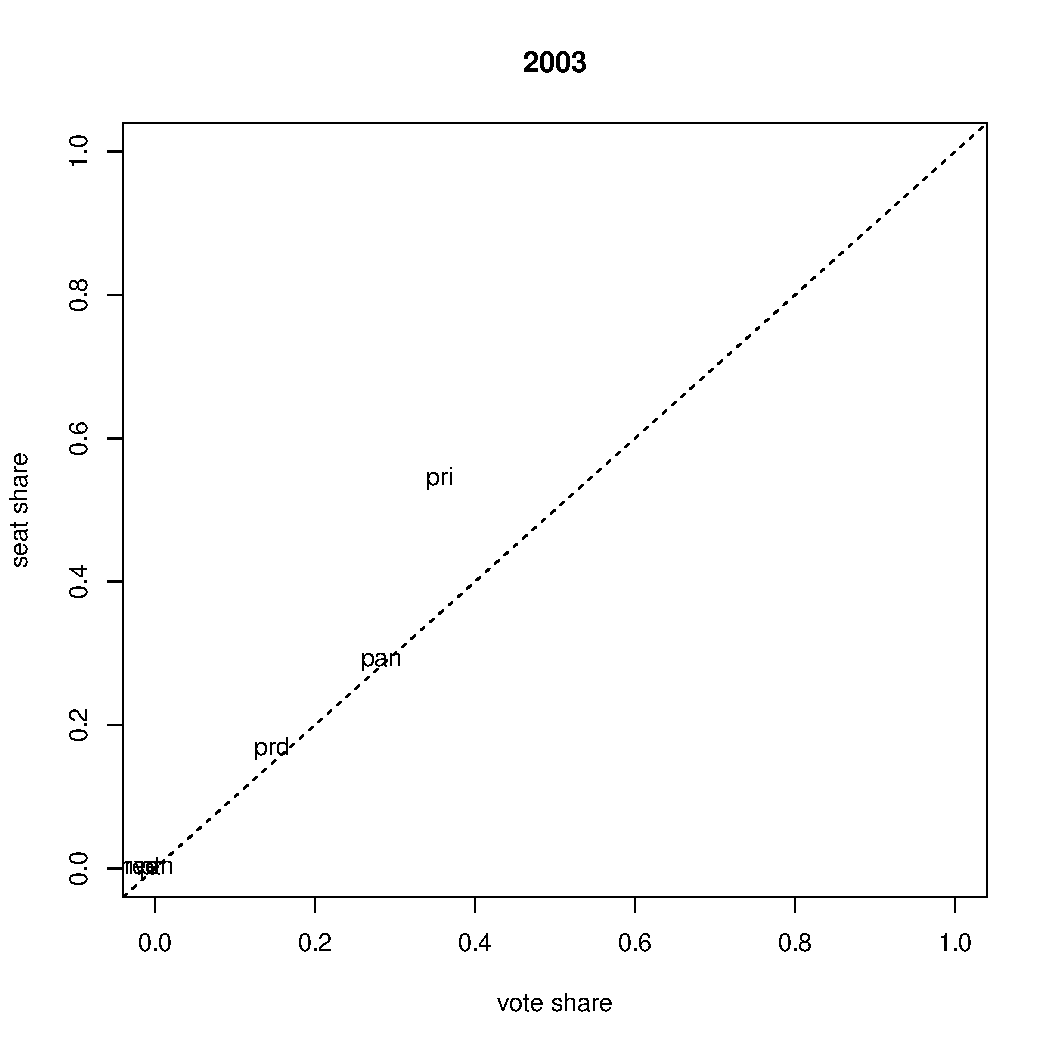
\includegraphics[width=.3\textwidth]{../../graphs/vsNosims2003.pdf} &
   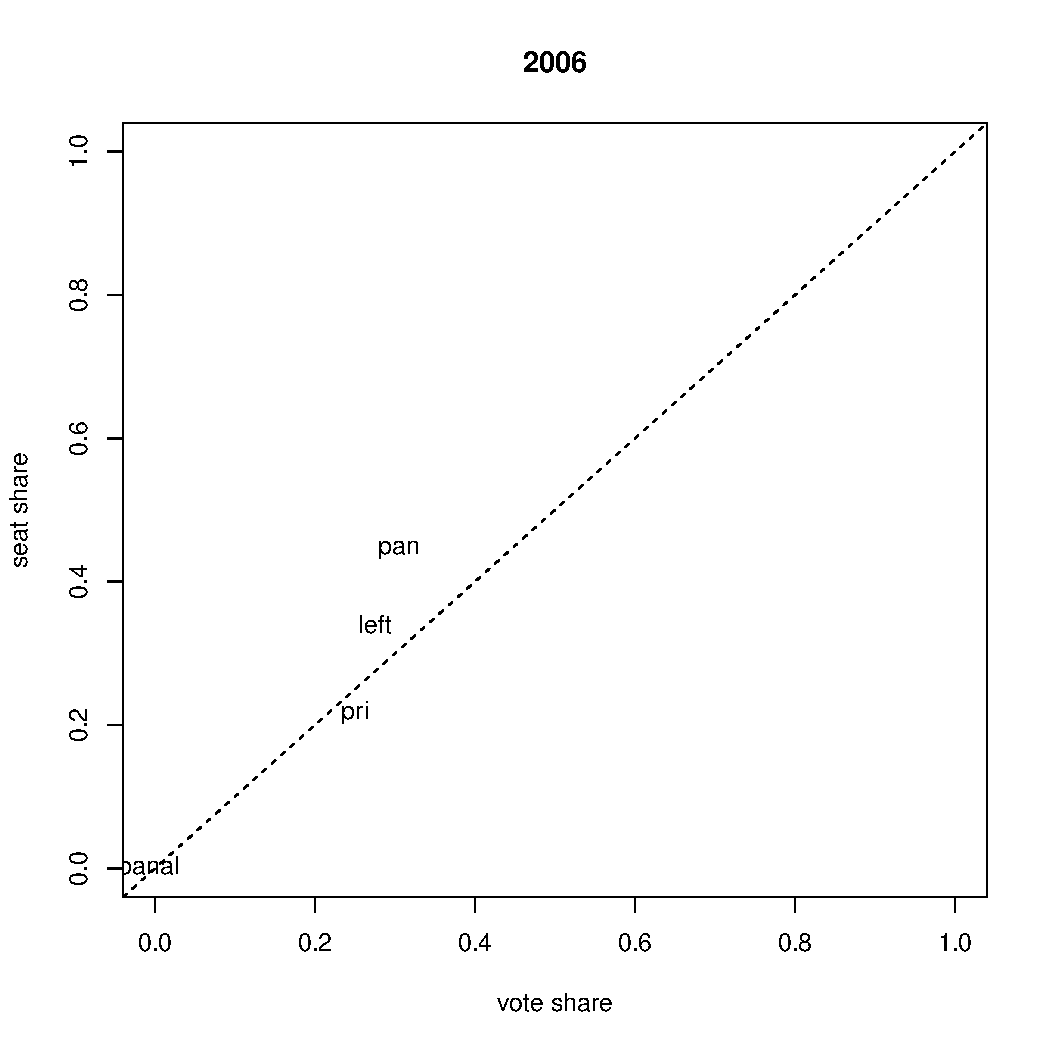
\includegraphics[width=.3\textwidth]{../../graphs/vsNosims2006.pdf} \\
   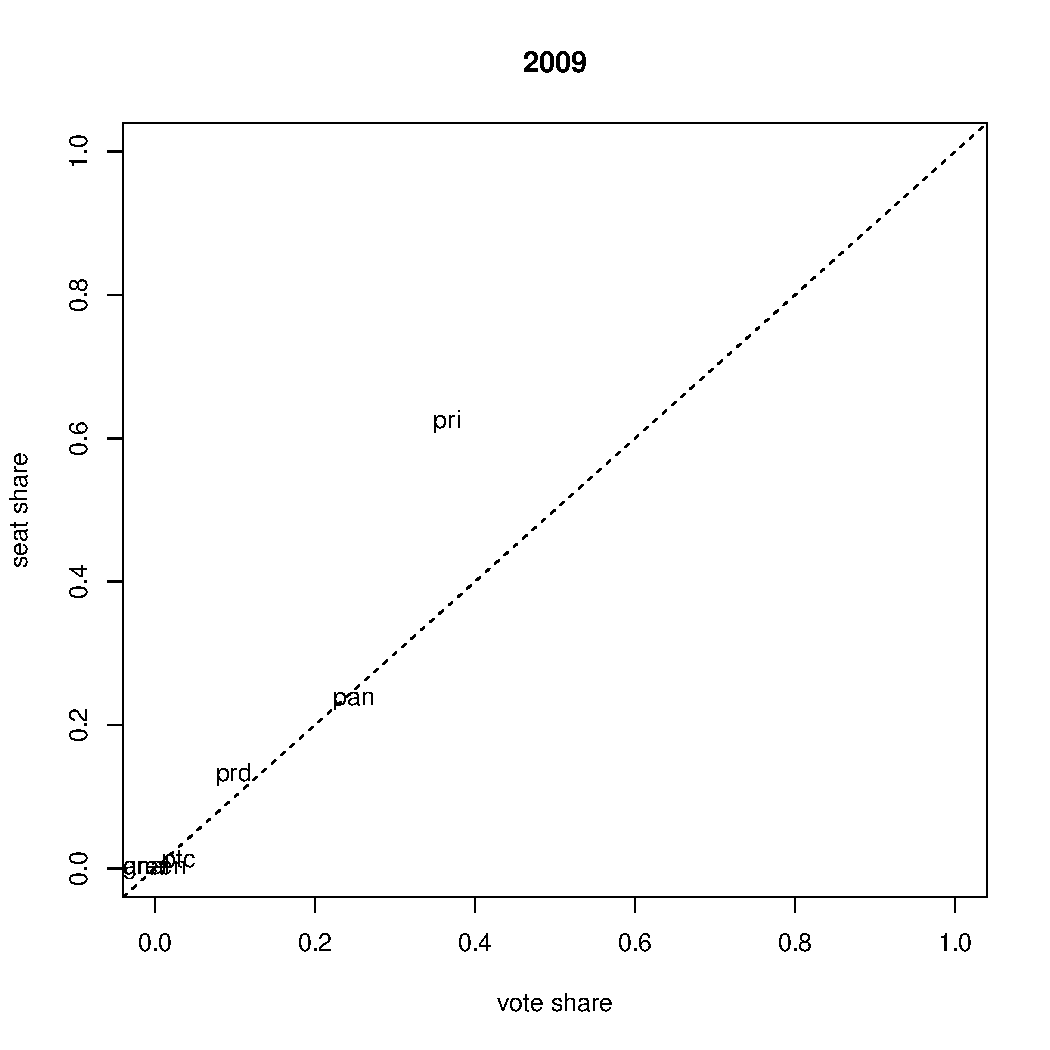
\includegraphics[width=.3\textwidth]{../../graphs/vsNosims2009.pdf} &
   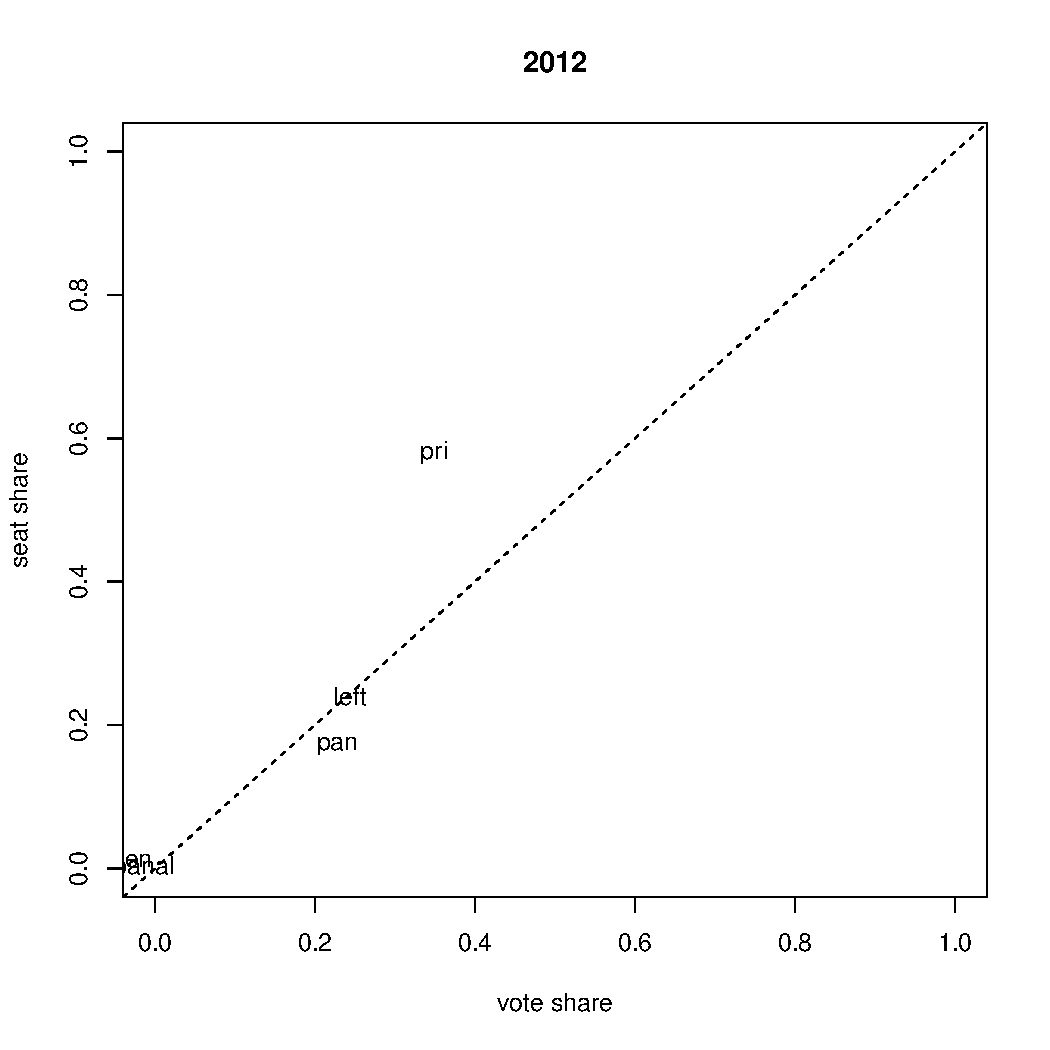
\includegraphics[width=.3\textwidth]{../../graphs/vsNosims2012.pdf} \\
\end{tabular}
\end{center}
}
%%%%%%%%%%%%%%%%%%%%%%%%%%%%%%%%%%%%%%%%%%%%%%%%%%%%%%%%%%%%%%%%%%%%%%%%%%%%%%%%%%%%%%%%%%%%
\frame {                      % SLIDE
    \frametitle{Obstacle 4: small-N}
\begin{itemize}
\item Linzer 2012: approximates prob.\ distribution of national party vote returns from observed district outcomes (FMM)
\item Use to simulate many elections w Monte Carlo draws
\end{itemize}

\begin{center}
\begin{tabular}{cc}
   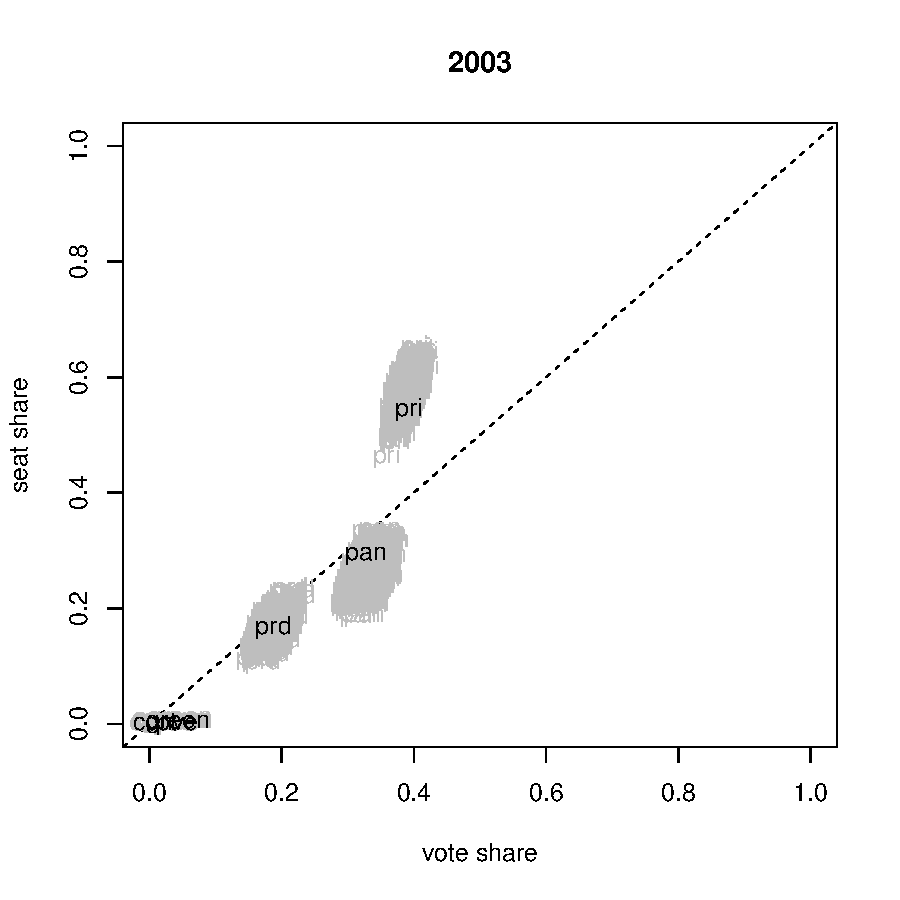
\includegraphics[width=.3\textwidth]{../../graphs/vs2003.pdf} &
   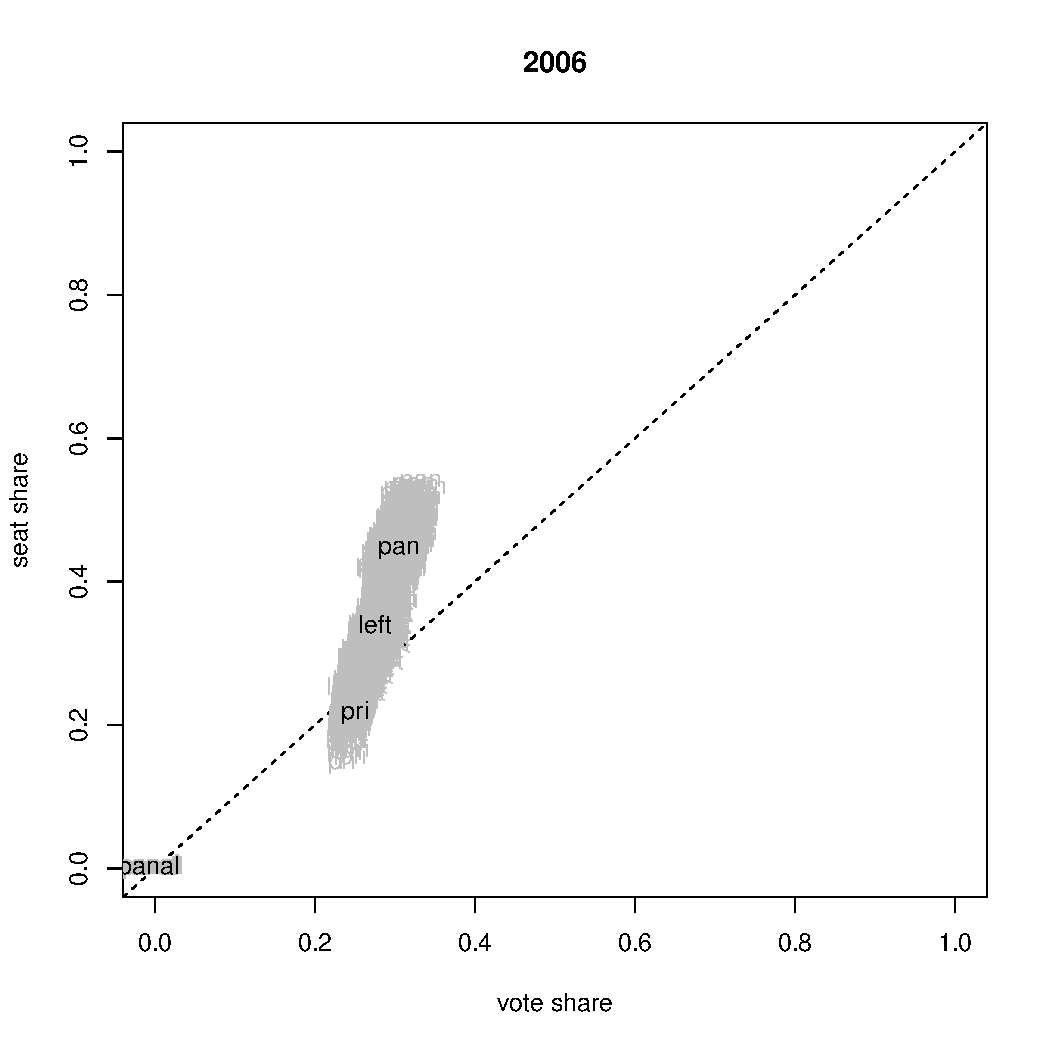
\includegraphics[width=.3\textwidth]{../../graphs/vs2006.pdf} \\
   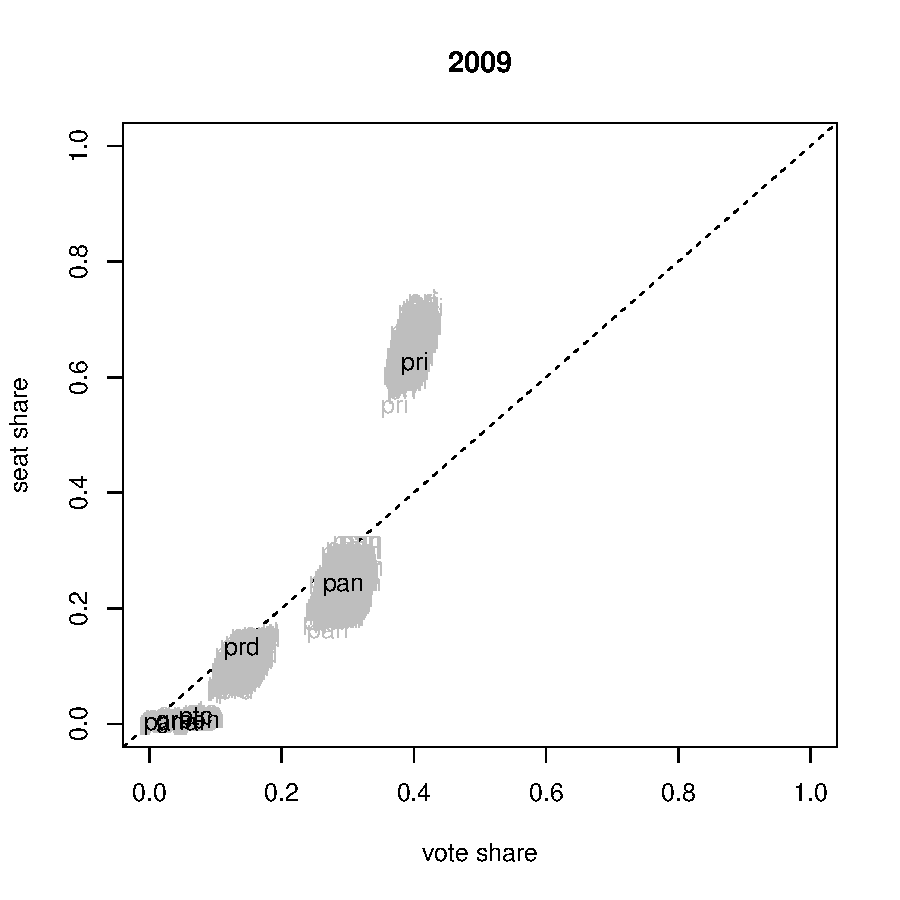
\includegraphics[width=.3\textwidth]{../../graphs/vs2009.pdf} &
   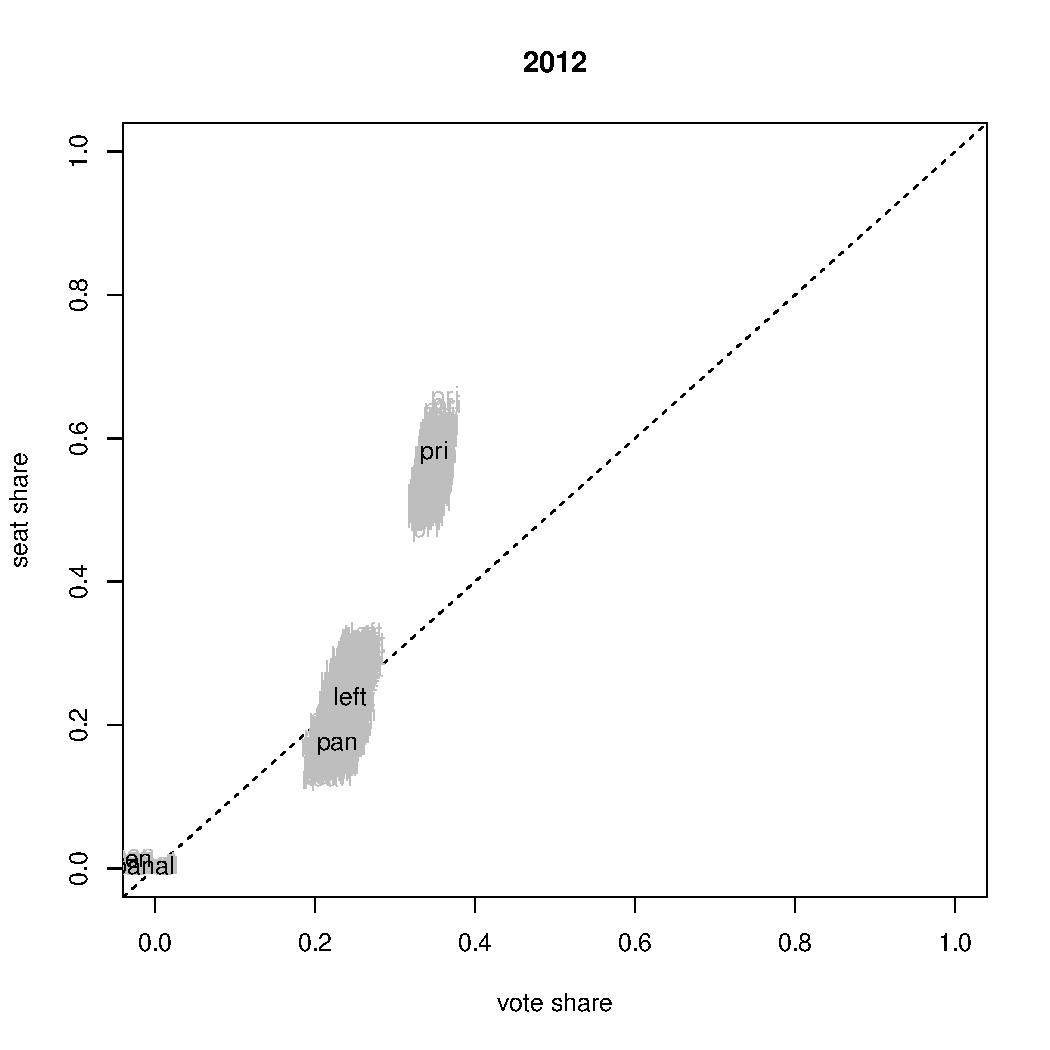
\includegraphics[width=.3\textwidth]{../../graphs/vs2012.pdf} \\
\end{tabular}
\end{center}
}
%%%%%%%%%%%%%%%%%%%%%%%%%%%%%%%%%%%%%%%%%%%%%%%%%%%%%%%%%%%%%%%%%%%%%%%%%%%%%%%%%%%%%%%%%%%% 
\frame{                      % SLIDE
    \frametitle{Two components 2009}

\begin{center}
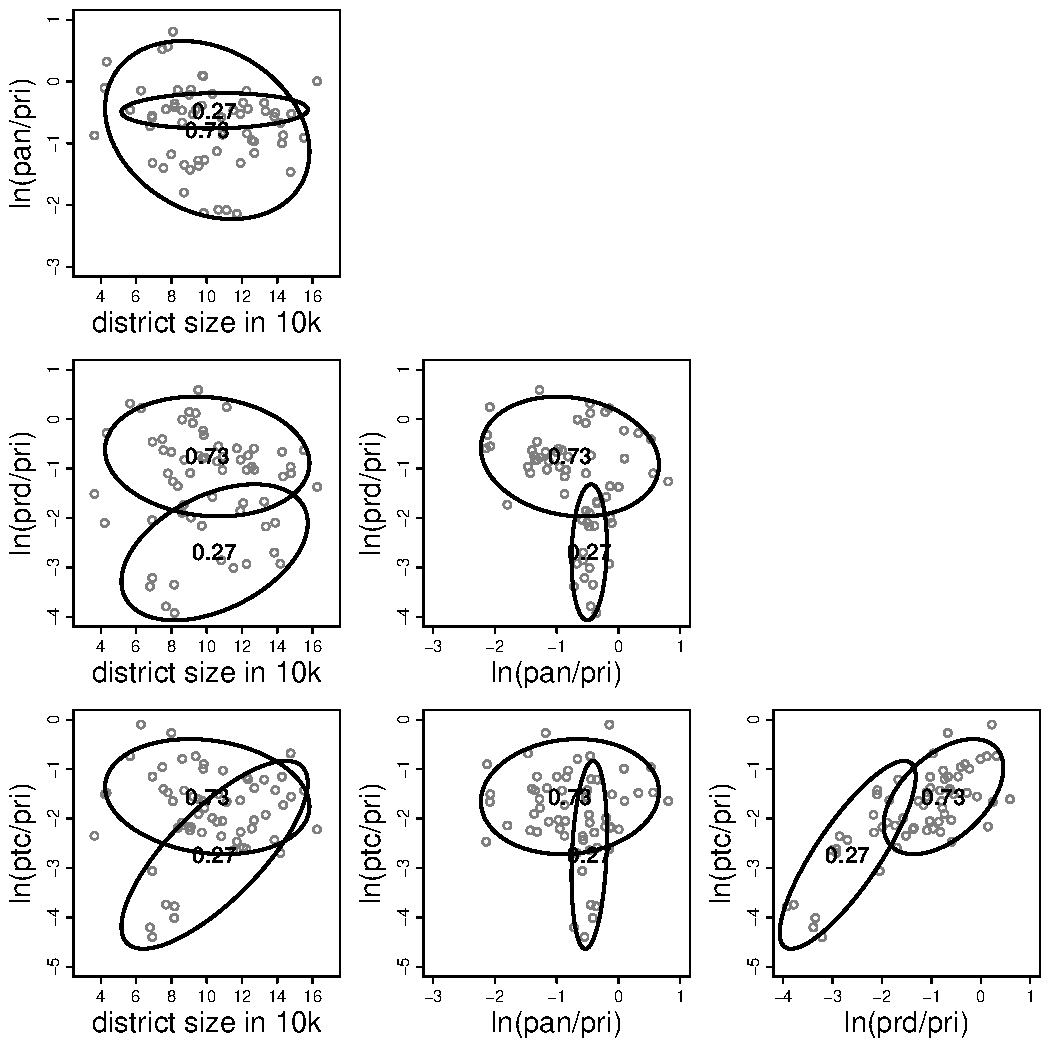
\includegraphics[width=.75\textwidth]{../../graphs/linzerLogVot2009-1.pdf} 
\end{center}
}
%%%%%%%%%%%%%%%%%%%%%%%%%%%%%%%%%%%%%%%%%%%%%%%%%%%%%%%%%%%%%%%%%%%%%%%%%%%%%%%%%%%%%%%%%%%% 
% \frame{                      % SLIDE
%     \frametitle{Conjectures}

% IFE is an agent of the major parties, power-sharing arrangement (Est\'evez, Magar, Rosas 2008)

% \bigskip

% \begin{enumerate}
% \item New map
% \end{enumerate}
% }
%%%%%%%%%%%%%%%%%%%%%%%%%%%%%%%%%%%%%%%%%%%%%%%%%%%%%%%%%%%%%%%%%%%%%%%%%%%%%%%%%%%%%%%%%%%% 
\frame{                      % SLIDE
    \frametitle{Results: raw party bias}

\centering
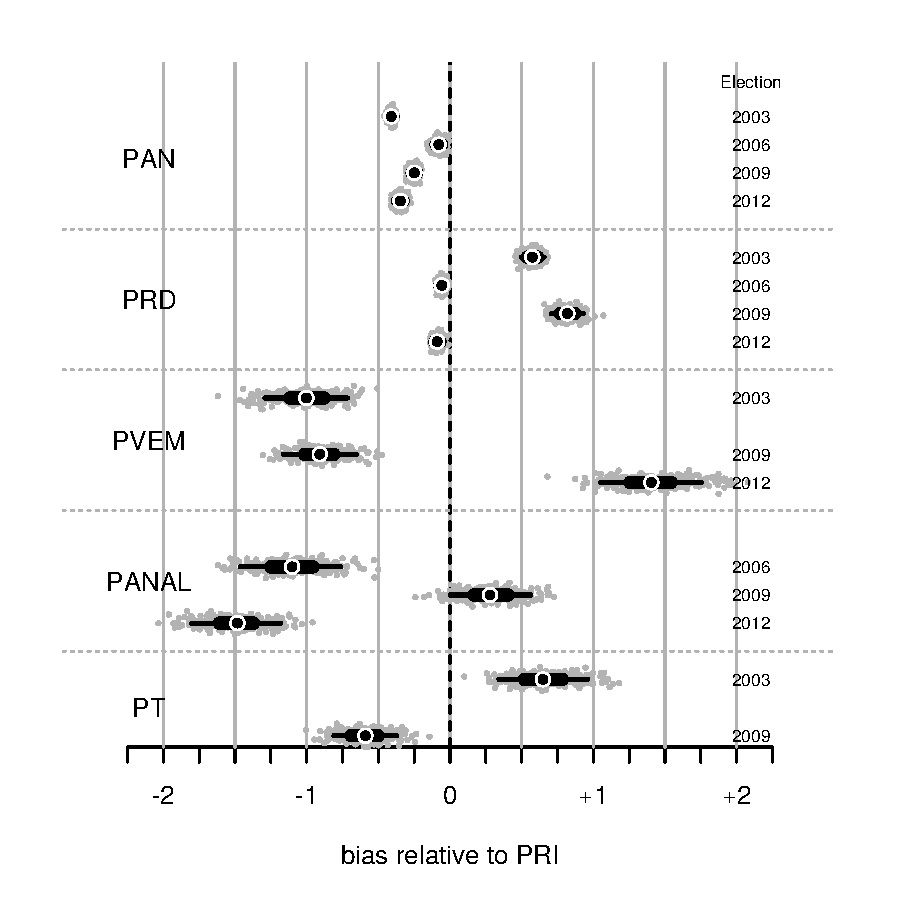
\includegraphics[width=.8\textwidth]{../../graphs/bias200612d0R.pdf} 

}
%%%%%%%%%%%%%%%%%%%%%%%%%%%%%%%%%%%%%%%%%%%%%%%%%%%%%%%%%%%%%%%%%%%%%%%%%%%%%%%%%%%%%%%%%%%% 
\frame{                      % SLIDE
    \frametitle{Results: components}

 \begin{columns}[c]

\column{.65\textwidth}

\newcommand{\mc}{\multicolumn}
\setbeamerfont{alerted text}{series=\bfseries} % makes alert boldface
%\newcolumntype{d}[1]{D{.}{.}{#1}} % D column with 1 decimal spaces default, usage d{2} for two spaces
%\newcolumntype{d}{D{.}{.}{2}} % D column with space for 2 decimal spaces
\resizebox{.95\textwidth}{!}{
\centering
\begin{tabular}{lrrr|rrr}
              &  \mc{3}{c|}{Actual map} & \mc{3}{c}{Hypothetical map} \\
party bias    &  \mc{1}{c}{\textsc{pan}--\textsc{pri}}  &  \mc{1}{c}{\textsc{prd}--\textsc{pri}} &  \mc{1}{c|}{min--\textsc{pri}}  & \mc{1}{c}{\textsc{pan}--\textsc{pri}}  &  \mc{1}{c}{\textsc{prd}--\textsc{pri}} &  \mc{1}{c}{min--\textsc{pri}} \\  \hline
\mc{4}{l}{\textbf{~2003 election}}     & \mc{3}{c}{(with 2006 map)} \\
raw           & $-$.37 &  +.72 &$-$1.01 &  $-$.41 &  +.57 &$-$1.00   \\ [-1ex]
              &   \mc{1}{r}{\footnotesize{(0)}}  &   \mc{1}{r}{\footnotesize{(0)}} &  \mc{1}{r|}{\footnotesize{(0)}}  &  \mc{1}{r}{\footnotesize{(0)}}  &   \mc{1}{r}{\footnotesize{(0)}} &  \mc{1}{r}{\footnotesize{(0)}}    \\
gerrym.       & $-$.09 &  +.69 &$-$.88 &  $-$.13 &  +.62 &$-$.90   \\ [-1ex]
              &   \mc{1}{r}{\footnotesize{(0)}}  &   \mc{1}{r}{\footnotesize{(0)}} &  \mc{1}{r|}{\footnotesize{(0)}}  &  \mc{1}{r}{\footnotesize{(0)}}  &   \mc{1}{r}{\footnotesize{(0)}} &  \mc{1}{r}{\footnotesize{(0)}}    \\
turnout       & \alert<2>{$-$.26} &\alert<2,5>{$-$.11} &\alert<2>{$-$.08} &  \alert<2>{$-$.26} &\alert<2>{$-$.09} &\alert<2>{$-$.09}   \\ [-1ex]
              &   \mc{1}{r}{\footnotesize{(0)}}  &   \mc{1}{r}{\footnotesize{(0)}} &  \mc{1}{r|}{\footnotesize{(0)}}  &  \mc{1}{r}{\footnotesize{(0)}}  &   \mc{1}{r}{\footnotesize{(0)}} &  \mc{1}{r}{\footnotesize{(0)}}    \\
malapp.       & $-$.01 &  \alert<3,5>{+.14} &$-$.05 &  \alert<4>{$-$.02} &  \alert<4>{+.05} &\alert<4>{$-$.02}   \\ [-1ex]
              &   \mc{1}{r}{\footnotesize{(.11)}}  &   \mc{1}{r}{\footnotesize{(0)}} &  \mc{1}{r|}{\footnotesize{(0)}}  &  \mc{1}{r}{\footnotesize{(.12)}} &   \mc{1}{r}{\footnotesize{(0)}} &  \mc{1}{r}{\footnotesize{(0)}}    \\
\mc{7}{l}{\textbf{~2006 election}}                                 \\
raw           & $-$.08 &$-$.06 & -1.10  &        &        &        \\ [-1ex]
              &   \mc{1}{r}{\footnotesize{(0)}}  &   \mc{1}{r}{\footnotesize{(0)}} &  \mc{1}{r|}{\footnotesize{(0)}}  & & & \\
gerrym.       &   \alert<5>{+.28} &  \alert<5>{+.30} &$-$.62  &        &        &        \\ [-1ex]
              &   \mc{1}{r}{\footnotesize{(0)}}  &   \mc{1}{r}{\footnotesize{(0)}} &  \mc{1}{r|}{\footnotesize{(0)}}  & & & \\
turnout       & \alert<2,5>{$-$.36} &\alert<2,5>{$-$.41} &\alert<2>{$-$.43}  &        &        &        \\ [-1ex]
              &   \mc{1}{r}{\footnotesize{(0)}}  &   \mc{1}{r}{\footnotesize{(0)}} &  \mc{1}{r|}{\footnotesize{(0)}}  & & & \\
malapp.       & $-$.00 &  \alert<3>{+.05} &$-$.05  &        &        &        \\ [-1ex]
              &   \mc{1}{r}{\footnotesize{(.42)}}  &   \mc{1}{r}{\footnotesize{(0)}} &  \mc{1}{r|}{\footnotesize{(0)}}  & & & \\
\mc{7}{l}{\textbf{~2009 election}}                                 \\ 
raw           & $-$.25 &  +.82 &$-$.91  &        &        &        \\  [-1ex]
              &   \mc{1}{r}{\footnotesize{(0)}}  &   \mc{1}{r}{\footnotesize{(0)}} &  \mc{1}{r|}{\footnotesize{(0)}}  & & & \\
gerrym.       & $-$.11 & \alert<5>{+1.01} &$-$.79  &        &        &        \\  [-1ex]
              &   \mc{1}{r}{\footnotesize{(0)}}  &   \mc{1}{r}{\footnotesize{(0)}} &  \mc{1}{r|}{\footnotesize{(0)}}  & & & \\
turnout       & \alert<2>{$-$.14} &\alert<2,5>{$-$.24} &\alert<2>{$-$.12}  &        &        &        \\  [-1ex]
              &   \mc{1}{r}{\footnotesize{(0)}}  &   \mc{1}{r}{\footnotesize{(0)}} &  \mc{1}{r|}{\footnotesize{(0)}}  & & & \\
malapp.       & $-$.00 &  \alert<3>{+.05} &$-$.00  &        &        &        \\  [-1ex]
              &   \mc{1}{r}{\footnotesize{(.36)}}  &   \mc{1}{r}{\footnotesize{(0)}} &  \mc{1}{r|}{\footnotesize{(0)}}  & & & \\
\mc{4}{l}{\textbf{~2012 election}}      & \mc{3}{c}{(with 2015 map)} \\
raw           & $-$.35 &$-$.09 & +1.40  &  $-$.32 &$-$.13 & +1.03  \\  [-1ex]
              &   \mc{1}{r}{\footnotesize{(0)}}  &   \mc{1}{r}{\footnotesize{(0)}} &  \mc{1}{r|}{\footnotesize{(0)}}  &  \mc{1}{r}{\footnotesize{(0)}}  &   \mc{1}{r}{\footnotesize{(0)}} &  \mc{1}{r}{\footnotesize{(0)}}    \\
gerrym.       & $-$.28 &$-$.07 & +1.41  &  $-$.24 &$-$.05 & +1.02  \\  [-1ex]
              &   \mc{1}{r}{\footnotesize{(0)}}  &   \mc{1}{r}{\footnotesize{(0)}} &  \mc{1}{r|}{\footnotesize{(0)}}  &  \mc{1}{r}{\footnotesize{(0)}}  &   \mc{1}{r}{\footnotesize{(.06)}} &  \mc{1}{r}{\footnotesize{(0)}}    \\
turnout       & \alert<2>{$-$.07} &\alert<2>{$-$.08} &  +.02  &  \alert<2>{$-$.08} &\alert<2>{$-$.09} &  +.01  \\  [-1ex]
              &   \mc{1}{r}{\footnotesize{(.02)}}  &   \mc{1}{r}{\footnotesize{(0)}} &  \mc{1}{r|}{\footnotesize{(0)}}  &  \mc{1}{r}{\footnotesize{(.26)}}  &   \mc{1}{r}{\footnotesize{(0)}} &  \mc{1}{r}{\footnotesize{(0)}}    \\
malapp.       &   +.01 &  \alert<3>{+.06} &$-$.02  &  \alert<4>{$-$.00} &  \alert<4>{+.01} &  \alert<4>{+.00}  \\  [-1ex]
              &   \mc{1}{r}{\footnotesize{(.42)}} &   \mc{1}{r}{\footnotesize{(0)}} &  \mc{1}{r|}{\footnotesize{(0)}}  &  \mc{1}{r}{\footnotesize{(.38)}}  &   \mc{1}{r}{\footnotesize{(0)}} &  \mc{1}{r}{\footnotesize{(0)}}    \\ \hline 
\end{tabular}
}

\column{.35\textwidth}

\begin{itemize}
\item<2-> Turnout always pro-PRI
\item<3-> Malapp.\ always pro-left
\item<4-> Redistricting abates malapp. 
\item<5-> Possibly cancelling effects 
\end{itemize}

\end{columns}

}
%%%%%%%%%%%%%%%%%%%%%%%%%%%%%%%%%%%%%%%%%%%%%%%%%%%%%%%%%%%%%%%%%%%%%%%%%%%%%%%%%%%%%%%%%%%%%%%%
\frame {                      % SLIDE
    \frametitle{Findings, next steps}

\begin{enumerate}

\item Rel.\ to the right, persistent pro-PRI, and esp.\ pro-left bias 

\item Though substantial malapportionent, effects are small

\item Gerrymandering effects large and volatile

\item Pro-PRI turnout-based bias  

\item District lines can compensate for turnout disadvantage

\item To-do: add PR-tier to analysis

\item To-do: study inter-election volatility

\end{enumerate}

\pause

\bigskip

\center{\textbf{\Large{Thank you!}}}

}
%%%%%%%%%%%%%%%%%%%%%%%%%%%%%%%%%%%%%%%%%%%%%%%%%%%%%%%%%%%%%%%%%%%%%%%%%%%%%%%%%%%%%%%%%%%% 
\frame{                      % SLIDE
    \frametitle{The redistricting process}
\begin{center}
   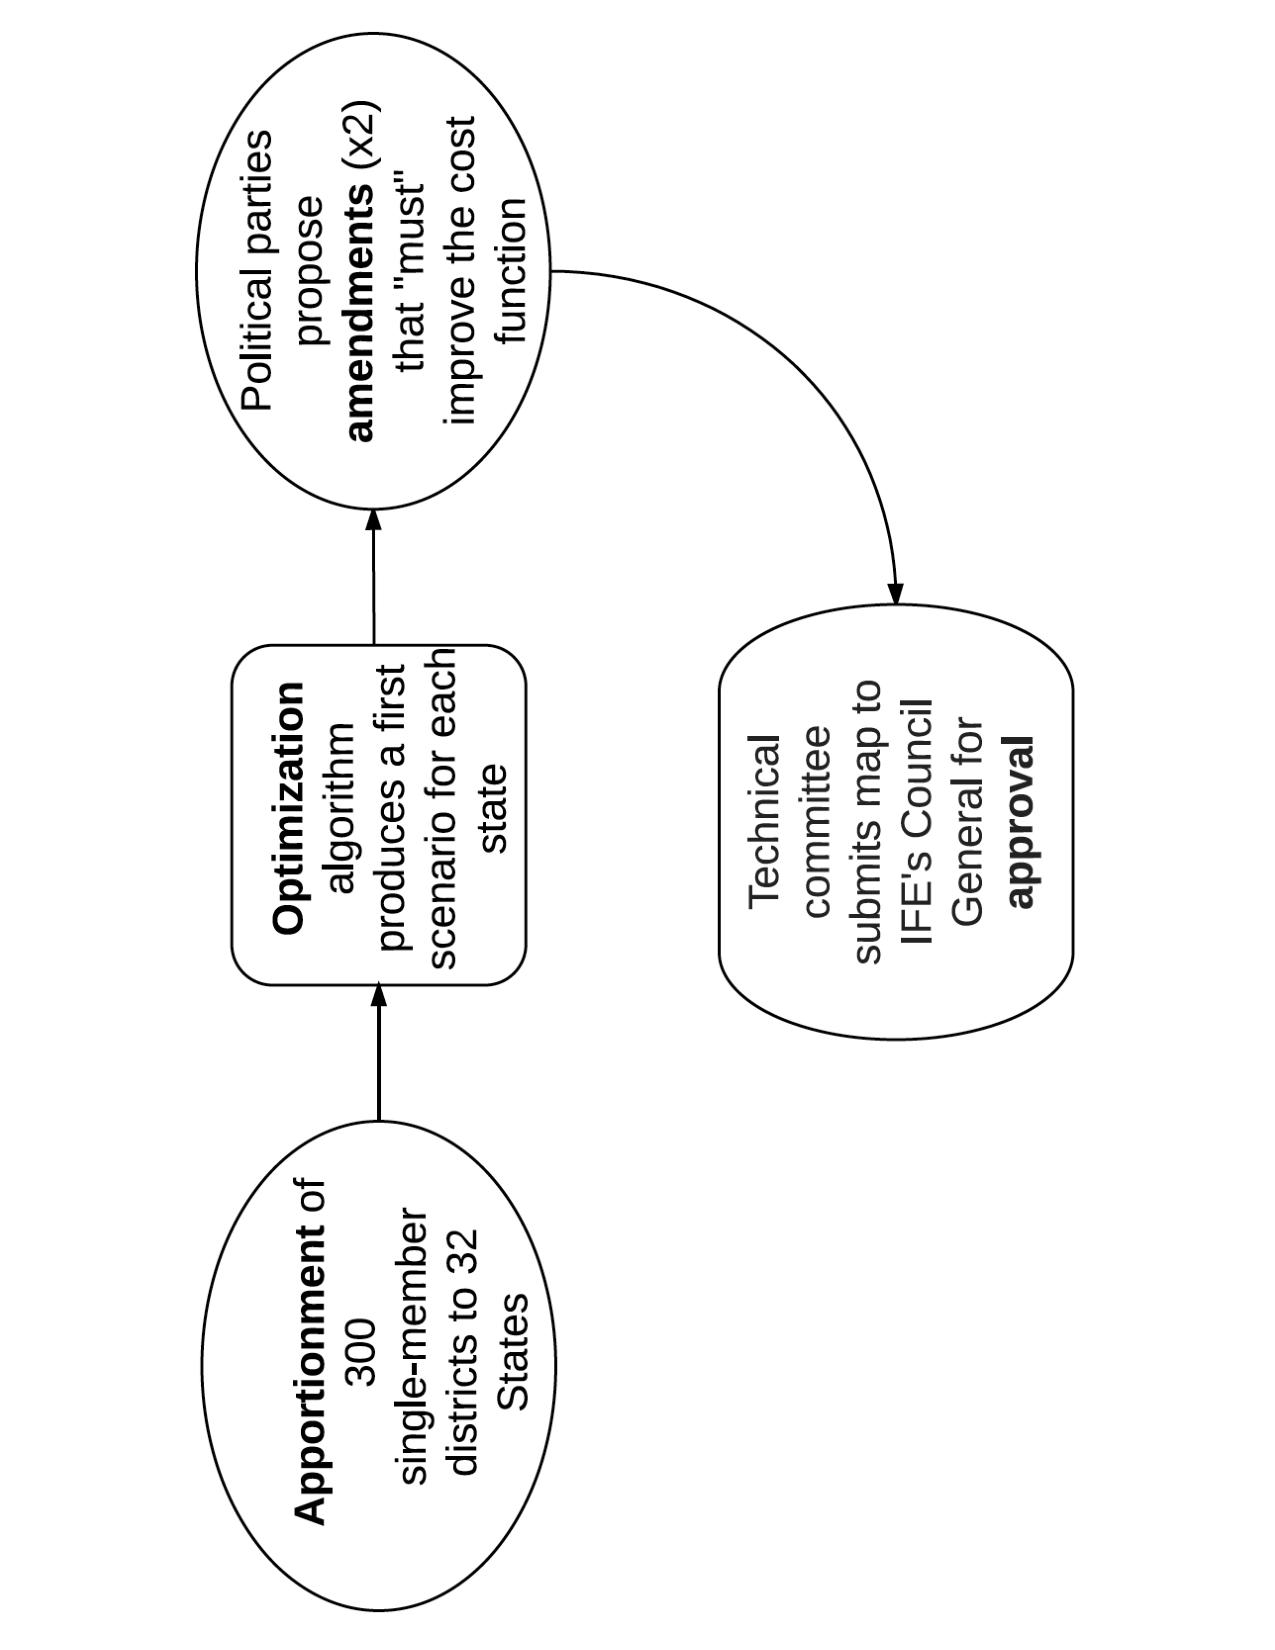
\includegraphics[width=8cm, angle=-90]{../../graphs/mexRedisProcessFlowchart.pdf}
\end{center}
}
%%%%%%%%%%%%%%%%%%%%%%%%%%%%%%%%%%%%%%%%%%%%%%%%%%%%%%%%%%%%%%%%%%%%%%%%%%%%%%%%%%%%%%%%%%%% 
\frame{                      % SLIDE
    \frametitle{The redistricting process}
Redistricting by experts in 1997, 2006, 2015 (abandoned), and now 2018

\begin{enumerate}
\item apportionment of 300 seats to 32 states
\item optimization algorithm $\rightarrow$ proposal
\item parties propose amendments (``must'' improve score)
%\item repeat 2 and 3
\item new map
\end{enumerate}

\begin{multline*}
\texttt{Score} = .4 \times \texttt{PopBalance} + .3 \times \texttt{MunicBoundaries} \\
+ .2 \times \texttt{TravelTime} + .1 \times \texttt{Compactness}
\end{multline*}

IFE considers $\pm15\%$ imbalance normal (!)
}
%%%%%%%%%%%%%%%%%%%%%%%%%%%%%%%%%%%%%%%%%%%%%%%%%%%%%%%%%%%%%%%%%%%%%%%%%%%%%%%%%%%%%%%%%%%% 
\frame{                      % SLIDE
    \frametitle{Optimization algorithm}
Simulated annealing = probabilistic meta-heuristic for optimization \\ locates a good approximation to the global optimum of the cost function in a large search space

\bigskip

Thousands of iterations using electoral \emph{secciones} 

\bigskip

Combinatorial optimization algorithm used to generate 
the first scenario in each state


\begin{center}
   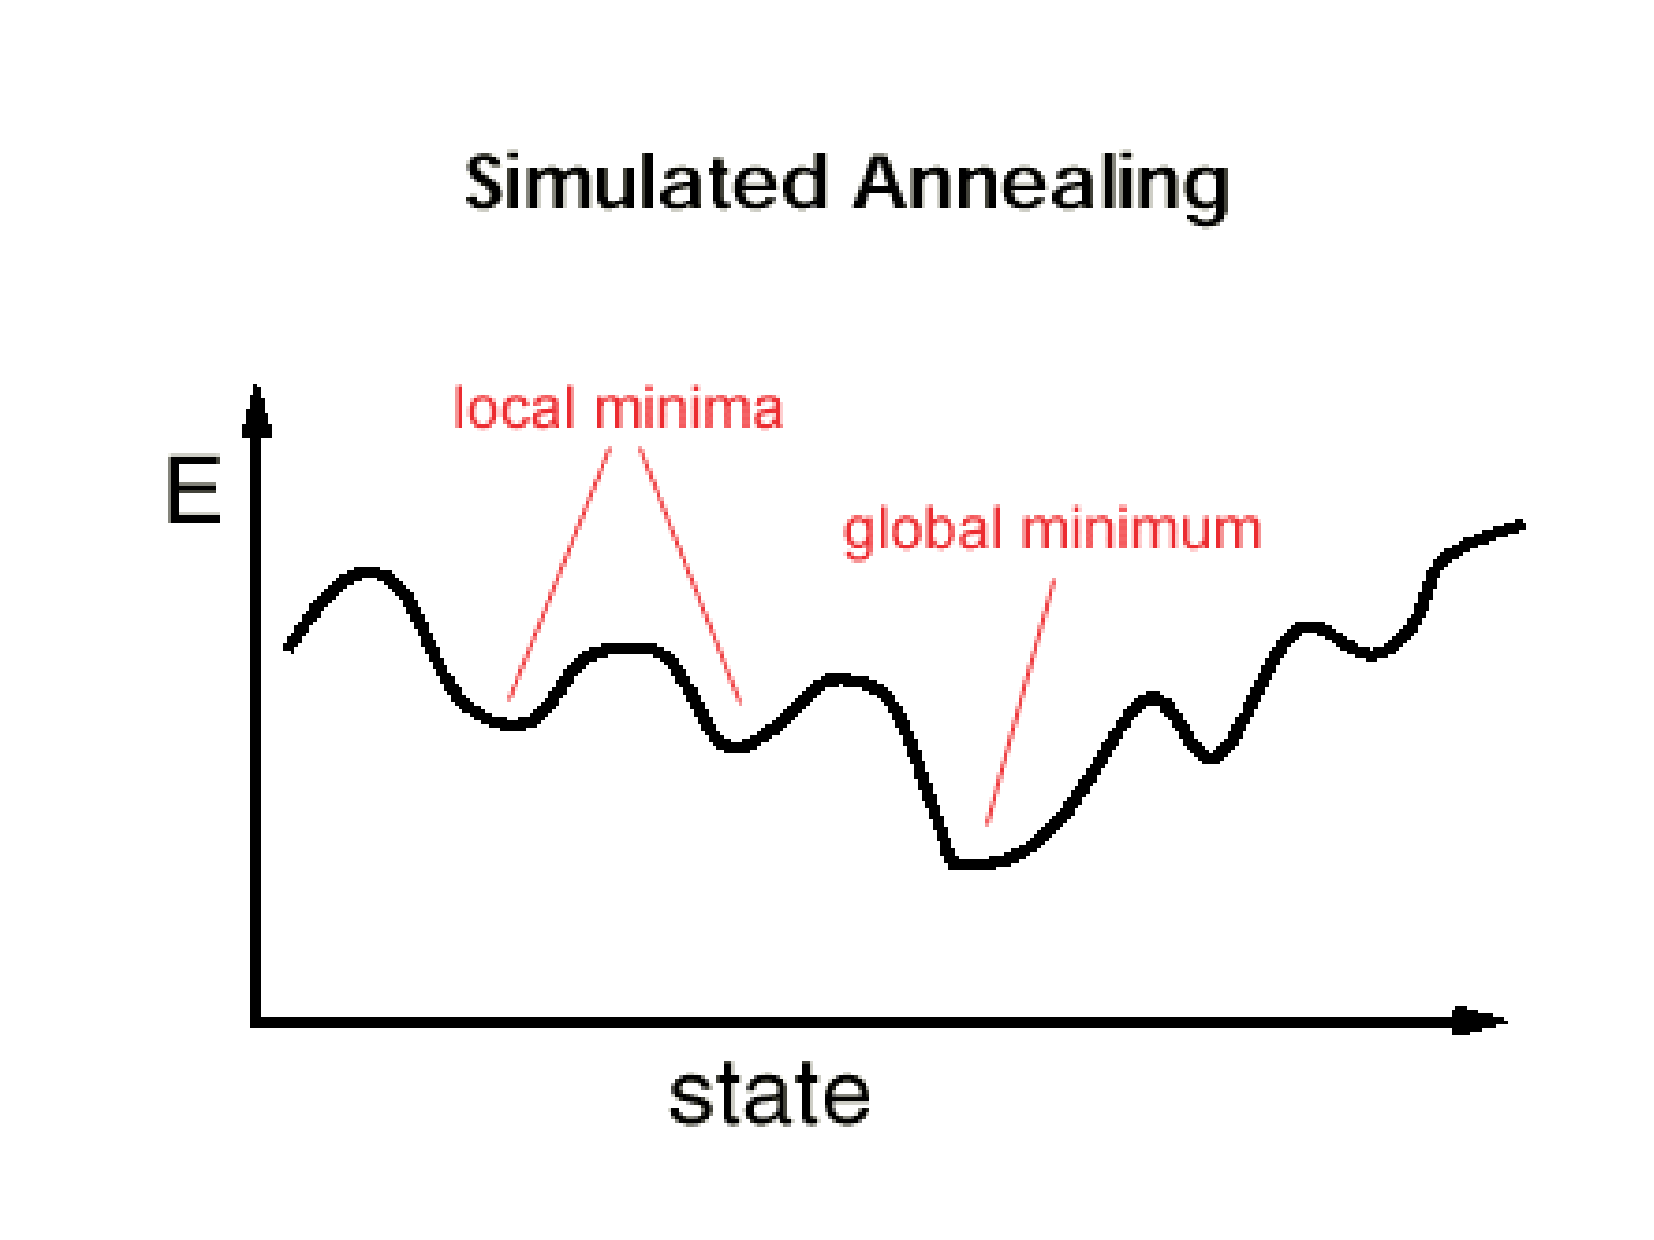
\includegraphics[width=5cm]{../../graphs/sim.pdf}
\end{center}

IFE claims that this is a public process, but the \\ operation and procedures are done \alert{behind closed doors}
}
%%%%%%%%%%%%%%%%%%%%%%%%%%%%%%%%%%%%%%%%%%%%%%%%%%%%%%%%%%%%%%%%%%%%%%%%%%%%%%%%%%%%%%%%%%%% 
\frame{                                       % SLIDE
    \frametitle{Party amendments}
\begin{center}
   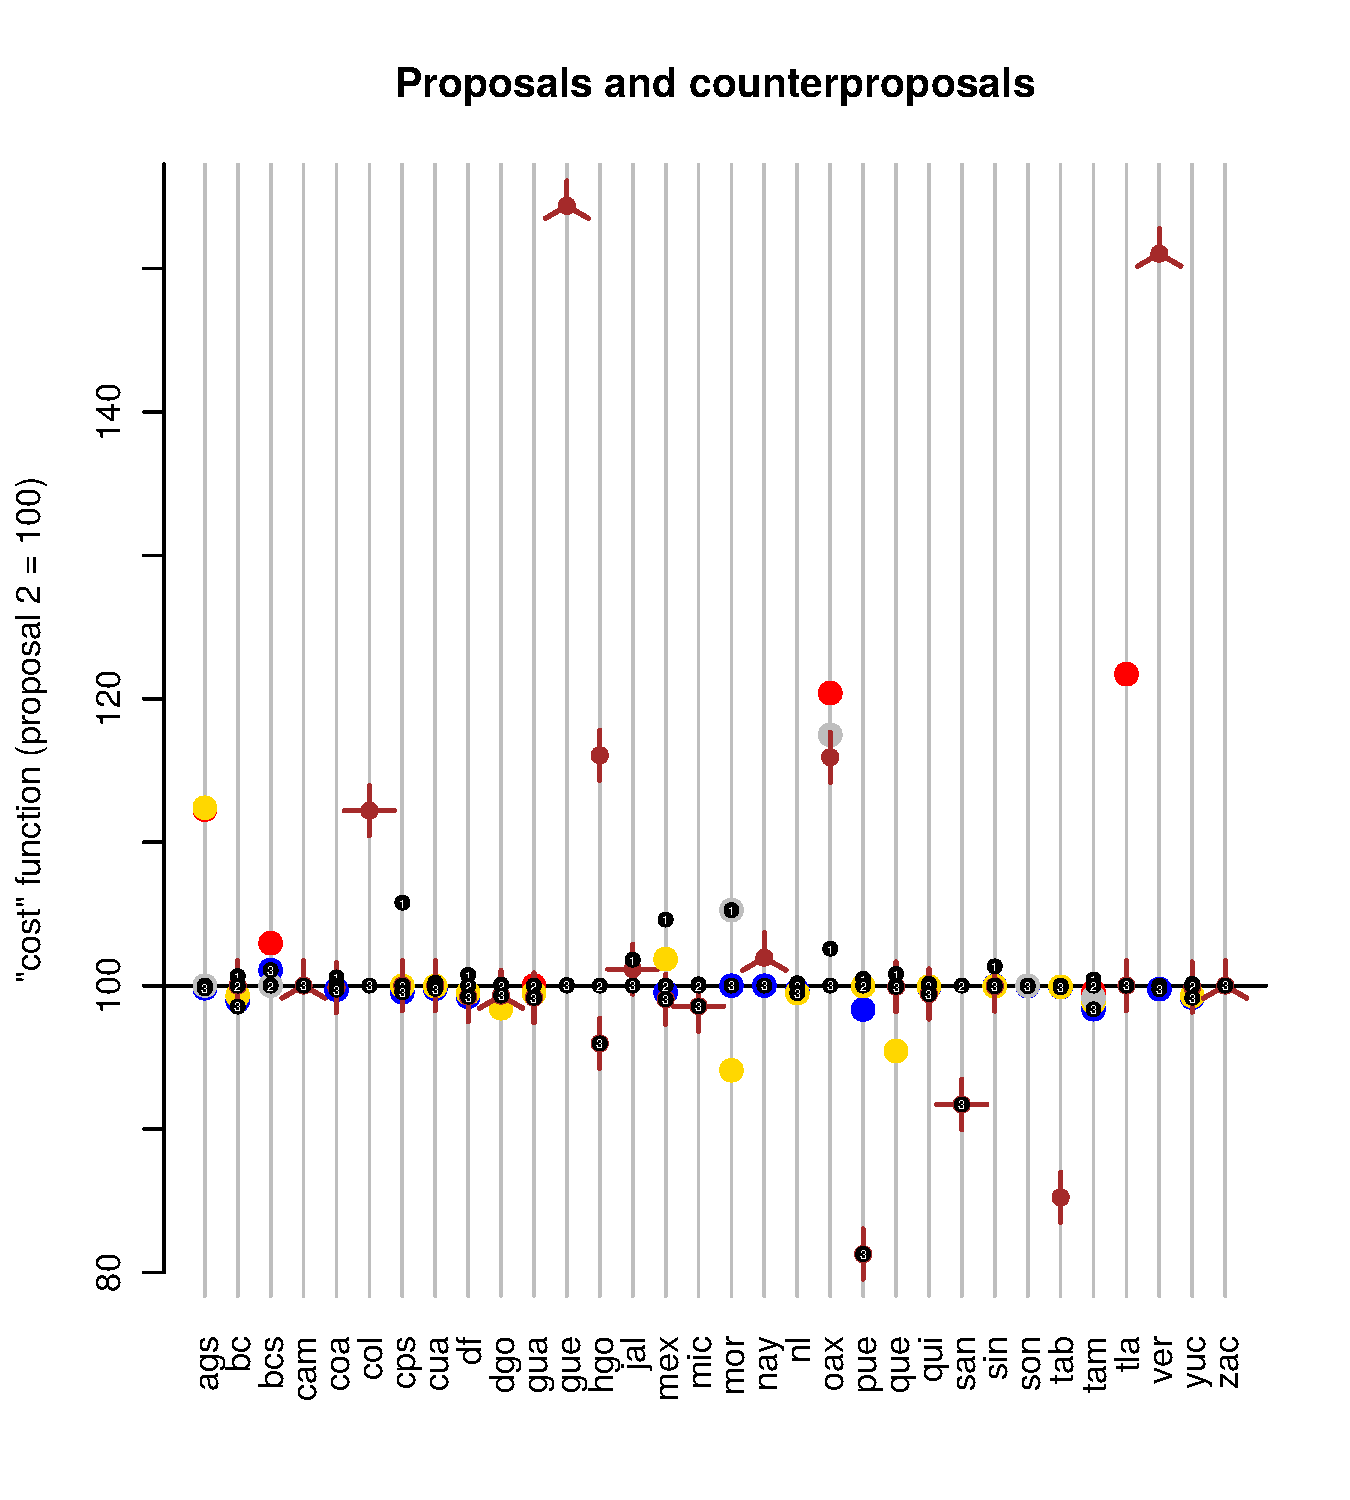
\includegraphics[width=8cm]{../../graphs/propsAndCost.pdf}
\end{center}
}
\end{document}
